\documentclass[conference]{IEEEtran}
\usepackage[utf8]{inputenc}
\usepackage[T1]{fontenc}
\usepackage{cite}
\usepackage{amsmath,amssymb}
\usepackage{graphicx}
\usepackage{booktabs}
\usepackage{array}
\usepackage{url}
\usepackage[hidelinks]{hyperref}
\usepackage{xcolor}
\graphicspath{{../results/}}

\begin{document}

\title{Nyaya-RAG: An Agentic Retrieval-Augmented Generation System for Indian Legal Document Analysis and Research}

\author{
\IEEEauthorblockN{Rajeev Ranjan}
\IEEEauthorblockA{Roll No. 240834\\
Indian Institute of Technology Kanpur\\
Kanpur, India\\
rajeev24@iitk.ac.in}
\and
\IEEEauthorblockN{Priyanshu Verma}
\IEEEauthorblockA{Roll No. 240811\\
Indian Institute of Technology Kanpur\\
Kanpur, India\\
priyanshuv24@iitk.ac.in}
\and
\IEEEauthorblockN{Sujal Kumar}
\IEEEauthorblockA{Roll No. 241050\\
Indian Institute of Technology Kanpur\\
Kanpur, India\\
sujalk24@iitk.ac.in}
}

\maketitle

\begin{abstract}
Legal research in India requires reading long Supreme Court judgments and locating the governing provision among thousands of statutory sections, at a time when the criminal codes themselves have been replaced. We present Nyaya-RAG, an agentic retrieval-augmented generation system built over 31,491 Supreme Court of India judgments and 39,967 sections of 1,034 Indian bare acts. The agent routes each query, retrieves evidence with a hybrid sparse-plus-dense retriever, generates an answer in which every sentence cites its source, verifies each claim against the cited source, and corrects itself when a claim is unsupported. On the Court Judgment Prediction and Explanation benchmark of the Indian Legal Documents Corpus (ILDC), the system predicts the outcome of 94.79\% of the 1,517 test cases, against 77.78\% for the best previously reported model, and its explanations overlap more with legal experts' annotations on four of six metrics. Hybrid retrieval ranks the correct statute section first for 69.6\% of curated questions, against 50.0\% for BM25 and 58.9\% for dense retrieval. The agentic pipeline raises answer faithfulness from 0.962 to 0.985 over a plain RAG baseline, and its self-check detects 41 of 42 injected hallucinations with no false alarm. Code and a live demonstration are publicly available.
\end{abstract}

\begin{IEEEkeywords}
retrieval-augmented generation, legal natural language processing, hybrid retrieval, judgment prediction, hallucination detection, large language models, Indian law
\end{IEEEkeywords}

\section{Introduction}
Indian courts carry a very large backlog of pending cases, and a single judgment of the Supreme Court of India commonly runs to several thousand words. A lawyer or student researching a point of law has to do three things: find the governing statutory provision, find how the Supreme Court has applied it, and judge how a new set of facts is likely to be decided. The task has recently become harder, because the Indian Penal Code, the Code of Criminal Procedure and the Indian Evidence Act were replaced in 2024 by the Bharatiya Nyaya Sanhita (BNS), the Bharatiya Nagarik Suraksha Sanhita (BNSS) and the Bharatiya Sakshya Adhiniyam (BSA), so that decades of case law refer to section numbers that no longer apply.

Large language models (LLMs) are an obvious aid, but they answer from parametric memory, cannot show where a statement comes from, and are known to fabricate legal authorities at high rates~\cite{dahl2024}. Retrieval-augmented generation (RAG)~\cite{lewis2020} addresses this by placing retrieved passages in the prompt, which grounds the answer in source text and makes it traceable.

Our starting point is the work of Malik \emph{et al.}~\cite{malik2021}, who introduced the Indian Legal Documents Corpus (ILDC) and the task of Court Judgment Prediction and Explanation (CJPE). Their best model, a hierarchical XLNet~\cite{yang2019} with a BiGRU, reaches 77.78\% accuracy, while human legal experts reach about 94\%. That line of work has three limits which we address: the models read 512 tokens at a time although the median judgment has about 2,200 words; each case is classified in isolation, without statute or precedent; and the system only predicts, so a user cannot ask a legal question and check the answer.

This paper makes the following contributions.
\begin{itemize}
\item An agentic RAG pipeline for Indian law with query routing, three retrieval tools, citation-grounded generation, claim-level self-evaluation and a corrective retrieval loop.
\item A hybrid retriever combining BM25~\cite{robertson2009} and dense embeddings~\cite{xiao2023} by reciprocal rank fusion~\cite{cormack2009}, which outperforms both of its components on statute retrieval.
\item A statute corpus in which each section of the repealed criminal codes is linked to its counterpart in the 2023 codes.
\item Precedent-augmented, prior-injected judgment prediction, evaluated on the full ILDC test set and on its expert annotations.
\item A two-signal hallucination detector, validated by injecting known errors into generated answers.
\item A leakage audit of the benchmark, with overlap between training and test data removed and accuracy also reported on a leak-filtered subset.
\end{itemize}

\section{Related Work}
\subsection{Legal judgment prediction}
ILDC~\cite{malik2021} contains about 35,000 Supreme Court of India judgments with the final order removed, and a test portion annotated with explanations by five legal experts. The authors evaluate classical models, sequence models and transformers such as BERT~\cite{devlin2019}, RoBERTa~\cite{liu2019} and XLNet~\cite{yang2019}, and obtain explanations from occlusion scores over chunks. Domain-specific pre-training has since been explored through LEGAL-BERT~\cite{chalkidis2020} and InLegalBERT~\cite{paul2023}, and the IL-TUR benchmark~\cite{joshi2024} collects CJPE together with other Indian legal tasks. These approaches fine-tune encoders with a limited input window. We instead use a long-context generative model with retrieved evidence and no task-specific training.

\subsection{Retrieval-augmented generation}
RAG~\cite{lewis2020} conditions generation on passages returned by a retriever. Sparse retrieval with BM25~\cite{robertson2009} matches query terms, while dense retrieval~\cite{karpukhin2020,reimers2019} matches meaning through learned embeddings; the BGE family~\cite{xiao2023} provides compact general-purpose encoders. Reciprocal rank fusion~\cite{cormack2009} combines rankings without score calibration. Recent work adds control to the pipeline: Self-RAG~\cite{asai2024} lets the model decide when to retrieve and critique its own output, and Corrective RAG~\cite{yan2024} evaluates retrieved documents and triggers further retrieval. Our corrective loop follows this direction but operates on the generated claims rather than on the retrieved documents.

\subsection{Evaluation and hallucination}
RAGAS~\cite{es2023} proposes reference-free metrics for RAG such as faithfulness and answer relevance, judged by an LLM. Dahl \emph{et al.}~\cite{dahl2024} document that general-purpose LLMs frequently hallucinate on legal queries, which motivates explicit verification in a legal assistant. Overlap between generated and reference text is commonly measured with ROUGE~\cite{lin2004}, which the ILDC authors also use for explanations.

\section{Background: Retrieval for Legal Text}
\label{sec:background}
A language model generates text from patterns learned in training and has no built-in way to consult a source. Asked for the punishment under a particular section, it produces the most plausible continuation, which may be wrong or out of date. In RAG, a retriever first searches a trusted collection for passages relevant to the question, and the model is instructed to answer only from those passages. In law this gives three benefits: the answer rests on the actual text of the statute or judgment, each statement can be traced to a source, and the collection can be updated without retraining. The retriever bounds the system: a section that is not retrieved cannot be cited.

\textbf{Sparse retrieval.} BM25 scores a document $d$ for a query $q$ as
\begin{equation}
\mathrm{BM25}(q,d)=\sum_{t\in q}\mathrm{IDF}(t)\,\frac{f_{t,d}\,(k_1+1)}{f_{t,d}+k_1\!\left(1-b+b\,\frac{|d|}{\mathrm{avgdl}}\right)},
\end{equation}
where $f_{t,d}$ is the frequency of term $t$ in $d$, $|d|$ the document length and $\mathrm{avgdl}$ the mean length. It is strong on exact legal terms such as ``anticipatory bail'' but fails when the question uses different words from the statute.

\textbf{Dense retrieval.} An encoder maps the query and each passage to vectors, and passages are ranked by cosine similarity. This handles paraphrase, such as ``fears arrest'' for ``apprehending arrest'', but can miss rare exact terms and treats section numbers as nearly meaningless.

\textbf{Hybrid retrieval.} We run both retrievers and fuse their rankings by reciprocal rank fusion,
\begin{equation}
\mathrm{RRF}(d)=\sum_{r\in\{\text{sparse},\,\text{dense}\}}\frac{1}{k+\mathrm{rank}_r(d)},\qquad k=60,
\end{equation}
over the top 40 results of each method. A passage ranked highly by either method, and especially by both, rises to the top.

\section{Data}
Table~\ref{tab:data} lists the corpora. All are derived from public datasets.

\begin{table}[t]
\caption{Corpora used in this work}
\label{tab:data}
\centering
\begin{tabular}{@{}p{3.6cm}p{2.1cm}p{2.0cm}@{}}
\toprule
Corpus & Size & Use \\
\midrule
ILDC training judgments & 31,491 cases, 183,351 chunks & Retrieval index, local models \\
ILDC test set & 1,517 cases & Prediction (never indexed) \\
Expert-annotated cases & 55 cases, 5 experts & Explanation quality \\
Bare acts & 1,034 acts, 39,967 sections & Statute retrieval \\
Curated queries & 74 (56 with gold section) & Retrieval and answer quality \\
\bottomrule
\end{tabular}
\end{table}

\textbf{Split reconstruction.} The public copy of ILDC has no split column. Its row counts match Table~1 of~\cite{malik2021} exactly (32,305 multi-train, 5,082 single-train, 1,517 test), so the splits were rebuilt from row order and verified against an independent list of test identifiers.

\textbf{Leakage control.} We removed duplicate judgments and every training case that shares an identifier or a text ending with a test case, which reduces the training pool from 37,387 to 31,491 cases. Test cases are never placed in the retrieval index.

\textbf{Statutes.} Two public collections of central acts were merged into one section-level table. Official mapping tables between the old and the new criminal codes were attached to 2,318 sections as cross-reference text, so that a section of the Indian Penal Code also names its BNS counterpart.

\textbf{Curated queries.} We wrote 74 evaluation queries: 56 plain-language statute questions with a known correct section, 8 case-law questions, 6 questions needing both statute and case law, 2 direct citation questions and 2 out-of-scope questions. Statute questions never mention the section number, and each gold section was checked against the indexed text.

\section{System Design}
Fig.~\ref{fig:arch} shows the pipeline. Each step is logged in a trace shown to the user.

\begin{figure*}[t]
\centering
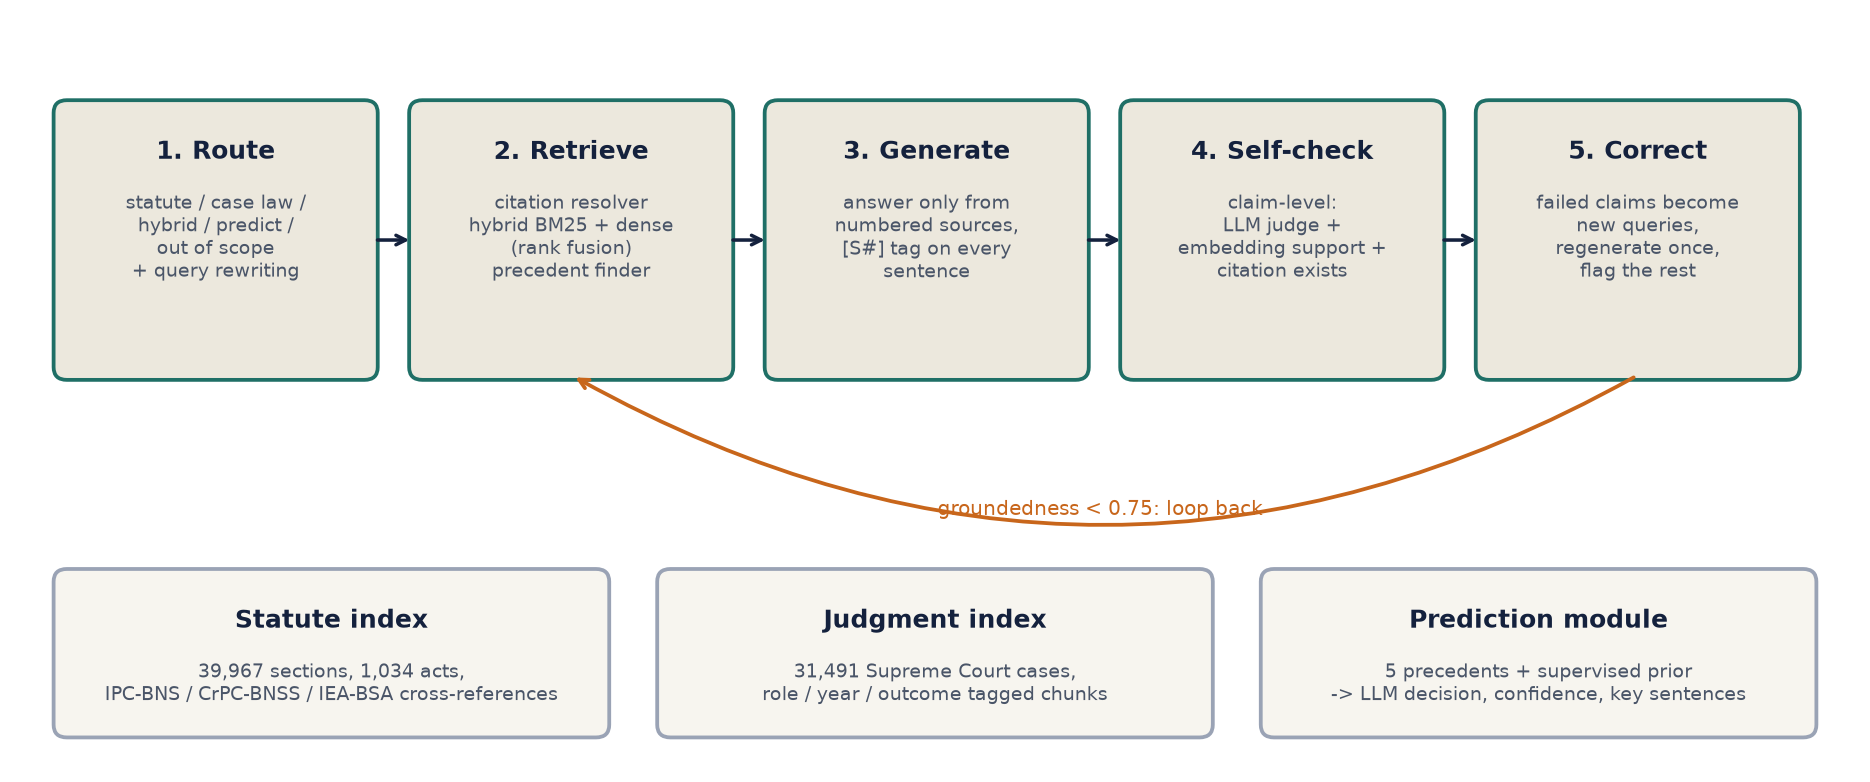
\includegraphics[width=0.92\textwidth]{fig_architecture.png}
\caption{Architecture of Nyaya-RAG. A query passes through routing, retrieval, citation-grounded generation and claim-level self-checking; unsupported claims trigger corrective retrieval.}
\label{fig:arch}
\end{figure*}

\subsection{Document-aware chunking and indexing}
Supreme Court judgments state facts and procedural history first and the Court's reasoning and conclusion last. Each judgment is split into 300-word windows aligned to the end of the document; the first two windows (facts) and the last six (reasoning) are kept, and every chunk is tagged with its role, case identifier, year and outcome. Statutes are chunked one section per chunk and never split. All chunks are embedded with \texttt{bge-small-en-v1.5} (384 dimensions) and indexed with BM25. A case-level vector, the mean of the reasoning-chunk embeddings, supports precedent search.

\subsection{Query router}
An LLM classifies the query as \emph{statute}, \emph{case law}, \emph{hybrid}, \emph{predict} or \emph{out of scope}, and rewrites it into one to three keyword-rich search queries with abbreviations expanded. The route selects the corpus to search; out-of-scope queries are declined.

\subsection{Retrieval tools}
\textbf{Citation resolver.} Queries such as ``Section 302 IPC'' or ``Article 21'' are resolved by pattern matching and an alias table directly to the exact section. Each section number is paired with the nearest act named in the query. No embedding is used, because section numbers carry no semantic content.

\textbf{Hybrid search.} BM25 and dense search are fused as in Section~\ref{sec:background}. For judgments, at most two chunks per case are kept so that one long case cannot fill the context.

\textbf{Precedent finder.} Given the text of a new case, it returns the nearest past judgments at case level together with their known outcomes.

\subsection{Citation-grounded generation}
The generator receives numbered sources and is instructed to answer only from them, to end every sentence stating law or fact with the tags of its supporting sources, to quote section numbers exactly, and to say plainly when the sources do not contain the answer.

\subsection{Self-evaluation}
The answer is split into claims, and each claim is checked in three ways: (i)~a claim citing a source number that does not exist is marked unsupported; (ii)~an LLM judge decides whether the cited sources fully support the claim, with verdicts \emph{supported}, \emph{partial} or \emph{unsupported}; (iii)~an embedding-support score is computed as the cosine similarity between the claim and the most similar sentence of its cited source. Groundedness is
\begin{equation}
G=\frac{1}{n}\sum_{i=1}^{n}s_i,\quad s_i=\begin{cases}1 & \text{supported}\\ 0.5 & \text{partial}\\ 0 & \text{otherwise.}\end{cases}
\end{equation}

\subsection{Corrective loop}
If $G<0.75$, the unsupported claims are used as new search queries, the new passages are added to the sources, and the answer is regenerated once with the failed claims as feedback. The better draft is kept and any claim that still fails is shown to the user with its verdict.

\subsection{Judgment prediction module}
For a pasted case the system retrieves the five most similar precedents and places the ending of each, with its outcome, in the prompt. A supervised prior is computed by a stack of three inexpensive local models trained on the training cases: TF-IDF with logistic regression on the last 1,024 words, a multilayer perceptron on the embeddings of the last six chunks, and a similarity-weighted vote of the 25 nearest precedents; the stacking weights are fitted on a held-out development set of 887 cases. The LLM reads the first 600 and the last 3,400 words of the case together with the precedents and the prior, and returns the appellant, a short reasoning, the decision, a confidence and up to eight sentences copied verbatim from the case. These sentences form the explanation.

\subsection{Implementation}
The system is written in Python. Retrieval, embeddings and the local models run on a laptop (Apple M4, 16\,GB). The LLM client supports several providers behind one interface, with a disk cache, rate limiting and model fallback. Experiments used Gemini 3.5 Flash-Lite and Gemini 3.1 Flash-Lite without fine-tuning. A Streamlit application exposes the agent with its trace, per-claim verdicts and sources.

\section{Experiments and Results}
\subsection{Judgment prediction}
Table~\ref{tab:pred} and Fig.~\ref{fig:pred} compare our system with the models reported in~\cite{malik2021} on the full ILDC test set. Nyaya-RAG reaches 94.79\% accuracy (95\% confidence interval 93.7 to 95.9), 17 points above the best reported model and on par with the human experts reported there.

\begin{table}[t]
\caption{Judgment prediction on the ILDC test set}
\label{tab:pred}
\centering
\begin{tabular}{@{}p{4.4cm}rr@{}}
\toprule
System & Acc. (\%) & Macro-F1 (\%) \\
\midrule
Doc2Vec + LR~\cite{malik2021} & 60.91 & 62.00 \\
XLNet, last 512 tokens~\cite{malik2021} & 70.01 & 71.07 \\
RoBERTa, last 512 tokens~\cite{malik2021} & 71.26 & 71.77 \\
XLNet + BiGRU (best)~\cite{malik2021} & 77.78 & 77.79 \\
Human experts~\cite{malik2021} & 93.93 & -- \\
\midrule
TF-IDF + LR (ours, local) & 67.96 & 67.18 \\
Stacked local prior (ours) & 68.16 & 68.14 \\
\textbf{Nyaya-RAG} & \textbf{94.79} & \textbf{94.79} \\
Nyaya-RAG + prior averaging & 94.86 & 94.85 \\
\bottomrule
\end{tabular}
\end{table}

\begin{figure}[t]
\centering
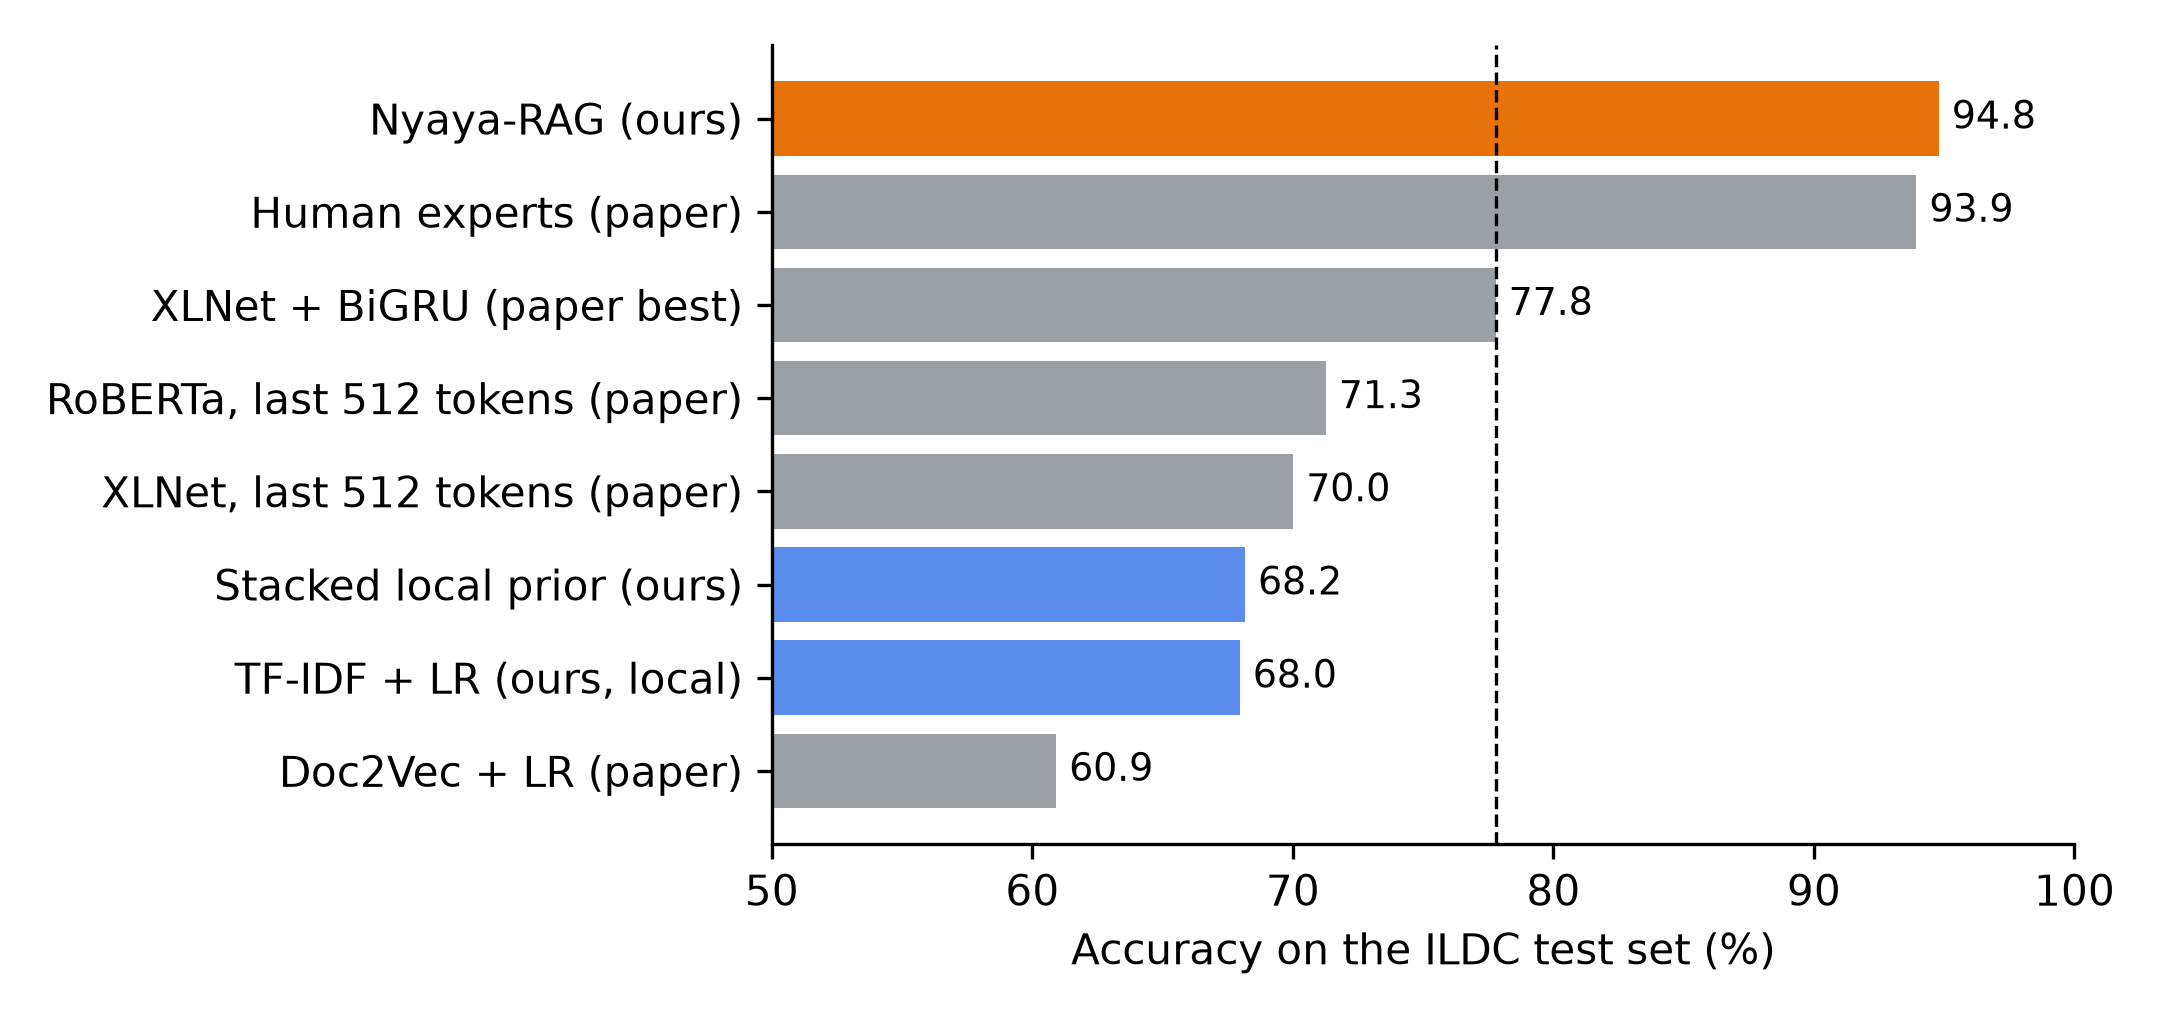
\includegraphics[width=\columnwidth]{fig_cjpe_paper.png}
\caption{Accuracy on the ILDC test set. Grey: reported in~\cite{malik2021}; blue: our local models; orange: Nyaya-RAG.}
\label{fig:pred}
\end{figure}

\textbf{Leakage check.} Some ILDC test documents still contain an explicit verdict phrase near the end. On the 1,364 test cases without such a phrase, accuracy is 94.72\%, so the result does not depend on leaked verdicts. In a further test, the last 150 words of each case were hidden, and 40 of 40 sampled cases were still predicted correctly. Of 3,034 model replies, 7 could not be parsed and are counted as wrong.

\textbf{Error analysis.} The errors we inspected were mostly cases in which the outcome label is itself debatable: appeals that are formally dismissed while the Court grants directions or modifies the decree, and cases in which several appeals are decided together. The ILDC authors report that their expert annotators disagreed with the official label on roughly 2 to 11\% of cases.

\subsection{Explanation quality}
Following~\cite{malik2021}, explanations are scored by their overlap with sentences highlighted by five legal experts. On 55 annotated cases the system selected about 11 sentences per case, of which 98\% appear verbatim in the judgment. Table~\ref{tab:exp} gives the mean over the five experts. Our explanations are closer to the experts on four metrics, level on ROUGE-1 and lower on ROUGE-L. ROUGE-L rewards sentence order, whereas the system lists sentences by importance. Jaccard and overlap are computed on word sets, which may differ slightly from the original definition.

\begin{table}[t]
\caption{Explanation overlap with legal experts (mean over five experts)}
\label{tab:exp}
\centering
\begin{tabular}{@{}lrr@{}}
\toprule
Metric & Ours & Occlusion~\cite{malik2021} \\
\midrule
ROUGE-1 & 0.457 & 0.451 \\
ROUGE-2 & \textbf{0.389} & 0.297 \\
ROUGE-L & 0.311 & \textbf{0.424} \\
Jaccard & \textbf{0.380} & 0.324 \\
Overlap-min & \textbf{0.875} & 0.719 \\
Overlap-max & \textbf{0.410} & 0.383 \\
\bottomrule
\end{tabular}
\end{table}

\subsection{Retrieval quality}
This experiment isolates the retriever. For each of the 56 statute questions we record the rank of the gold section among all 39,967 sections; no LLM is involved. Table~\ref{tab:ret} and Fig.~\ref{fig:ret} show that hybrid retrieval improves Hit@1 by 20 points over BM25 and 11 points over dense retrieval. The two methods fail on different questions: BM25 misses paraphrased questions and dense retrieval misses questions that hinge on an exact legal term. When the official BNS, BNSS or BSA counterpart of the gold section is also accepted, hybrid Hit@1 is 0.821.

\begin{table}[t]
\caption{Statute retrieval on 56 curated questions}
\label{tab:ret}
\centering
\begin{tabular}{@{}lrrrr@{}}
\toprule
Retriever & Hit@1 & Hit@3 & Hit@5 & MRR@10 \\
\midrule
BM25 & 0.500 & 0.804 & 0.857 & 0.661 \\
Dense (bge-small) & 0.589 & 0.875 & 0.911 & 0.734 \\
\textbf{Hybrid (RRF)} & \textbf{0.696} & \textbf{0.911} & \textbf{0.929} & \textbf{0.809} \\
\bottomrule
\end{tabular}
\end{table}

\begin{figure}[t]
\centering
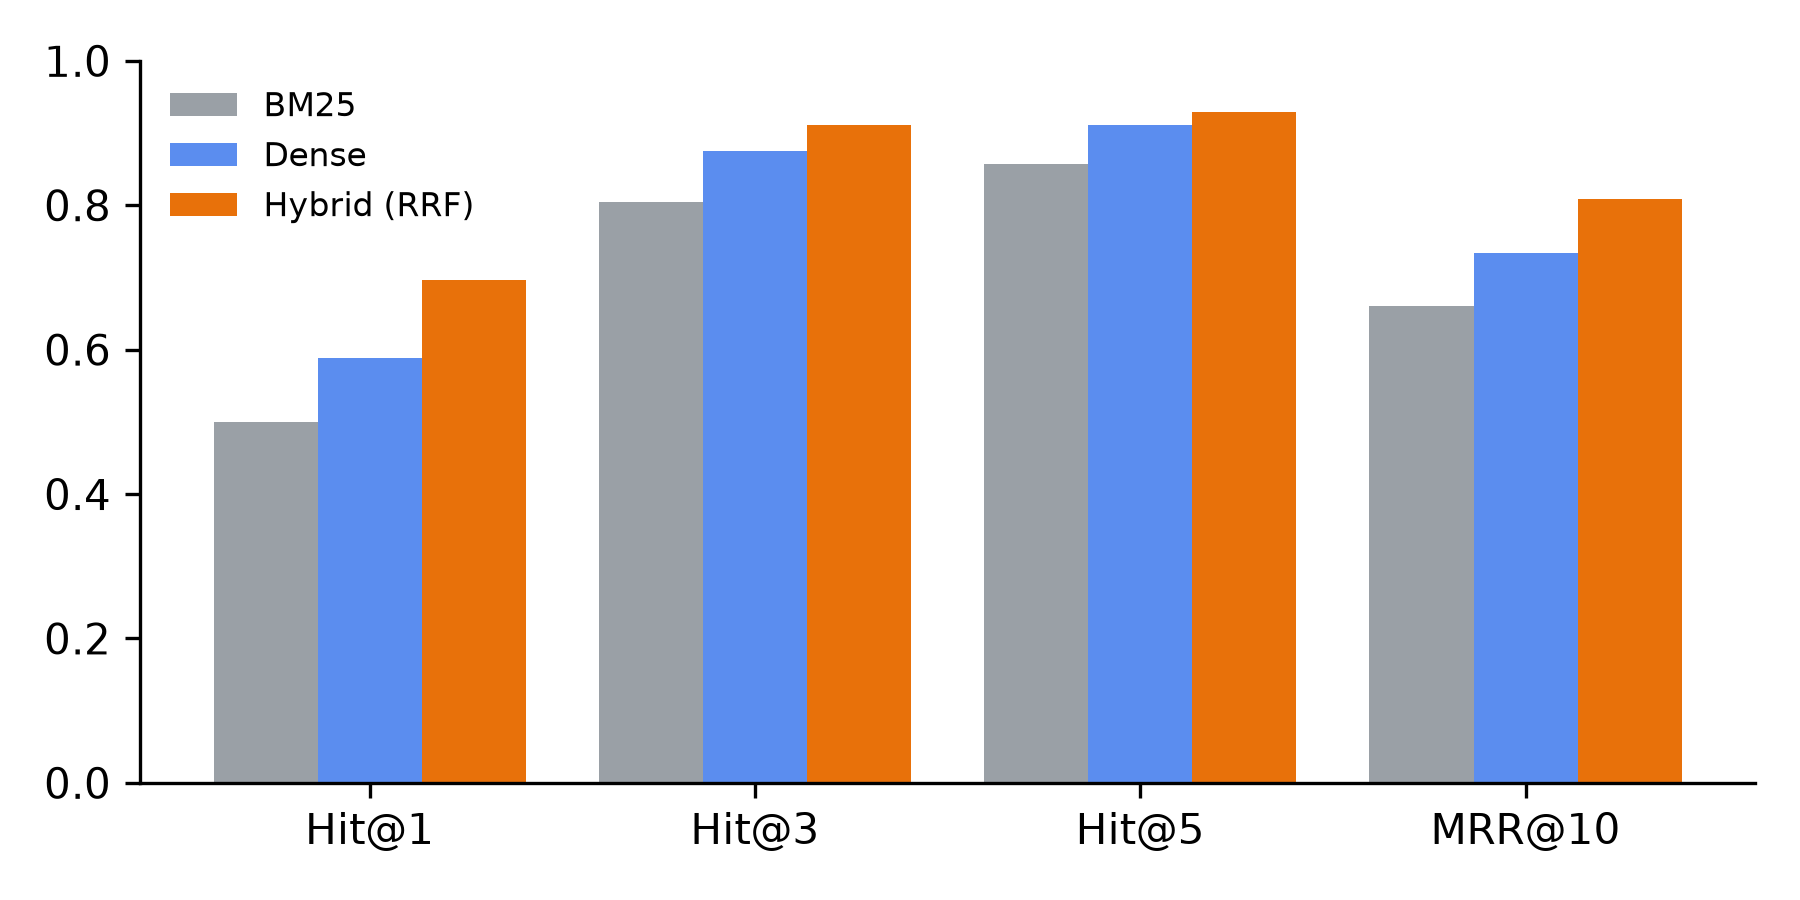
\includegraphics[width=0.9\columnwidth]{fig_retrieval_paper.png}
\caption{Statute retrieval: BM25, dense and hybrid.}
\label{fig:ret}
\end{figure}

\subsection{End-to-end answer quality}
We compare the full agentic pipeline with a plain RAG baseline (one dense retrieval followed by generation) on 46 of the curated queries, using RAGAS-style metrics~\cite{es2023} judged by an LLM. Table~\ref{tab:rag} shows that better retrieval carries through to the answers: the agentic pipeline cites the correct section more often and its answers are more faithful to their sources, with answer relevance essentially unchanged. The router chose an acceptable route for all 46 queries and declined both out-of-scope questions. The corrective loop fired once and raised that answer's groundedness from 0.71 to 1.0.

\begin{table}[t]
\caption{End-to-end answer quality on 46 curated queries}
\label{tab:rag}
\centering
\begin{tabular}{@{}lrr@{}}
\toprule
Metric & Plain RAG & Agentic (ours) \\
\midrule
Faithfulness & 0.962 & \textbf{0.985} \\
Citation validity & 0.983 & \textbf{0.990} \\
Answer relevance & \textbf{0.983} & 0.977 \\
Gold section cited & 0.893 & \textbf{0.929} \\
\bottomrule
\end{tabular}
\end{table}

As an example, for the question ``What is the law on anticipatory bail and what factors has the Supreme Court said courts should consider?'' the router chose the hybrid route. The answer cited Section~438 of the Code of Criminal Procedure and its successor, Section~482 of the BNSS, for the statutory rule, and a 2015 Supreme Court judgment for the factors, and every claim was judged supported.

\subsection{Hallucination detection}
To test the self-check, we took claims it had accepted as supported, corrupted one fact in each by program, and ran the check again. Table~\ref{tab:hal} shows that 41 of 42 injected errors (97.6\%) were detected, and none of the untouched claims in the same answers was wrongly flagged. The embedding-support score fell by only 0.019 on average for corrupted claims: similarity alone cannot detect a changed number or a negation, and the LLM judge is the component that detects errors.

\begin{table}[t]
\caption{Detection of injected hallucinations}
\label{tab:hal}
\centering
\begin{tabular}{@{}lr@{}}
\toprule
Injected error & Detected \\
\midrule
Wrong section or article number & 15 / 15 \\
Wrong duration & 4 / 4 \\
Flipped polarity or outcome & 22 / 23 \\
\midrule
Total & 41 / 42 \\
\bottomrule
\end{tabular}
\end{table}

\section{Discussion}
Reading the facts and the Court's reasoning together, with evidence in the prompt, closes the gap to the human experts reported for this benchmark, without any training on ILDC. Among the retrieval components, the move from a single method to hybrid retrieval is the largest measured gain, and it carries through to more correct citations and more faithful answers. Legal retrieval needs both exact and semantic matching, because statutory language is formulaic while users ask in everyday words. Section numbers are best handled symbolically, and the cross-references between the old and the new codes let the system answer questions phrased in either. Finally, verification has to be done by a model that reads the source: embedding similarity is not a substitute.

\section{Limitations and Future Work}
Prediction covers the full test set, but end-to-end answer quality was run on 46 of the 74 curated queries and the hidden-ending test on 40 cases. Supreme Court judgments are public, so the LLM may have seen some test cases in training; a test on judgments published after the model's training cut-off would settle this. Faithfulness and relevance are judged by the same model family that generated the answers, and a human-rated subset would be stronger. Prediction and explanation used Gemini 3.5 Flash-Lite, while answer quality, the hallucination test and the hidden-ending test used Gemini 3.1 Flash-Lite. The judgment corpus stops at 2020, carries ILDC identifiers rather than case names, and contains transcription artefacts. The system is a research aid and not legal advice. Future work includes High Court judgments, precedent retrieval by legal issue and by the appellant's position, a cross-encoder reranker, and evaluation with practising lawyers.

\section{Conclusion}
We presented Nyaya-RAG, an agentic RAG system for Indian legal research that combines hybrid retrieval over statutes and Supreme Court judgments with citation-grounded generation and claim-level self-verification. On the ILDC benchmark it predicts 94.79\% of test cases correctly against 77.78\% for the best previously reported model, its hybrid retriever outperforms sparse and dense retrieval alone, and its self-check detects nearly all injected hallucinations.

\section*{Code and Demo Availability}
Source code, evaluation scripts, the curated query set and all result files are available at \url{https://github.com/Sujal7508/nyaya-rag}. A live demonstration is hosted at \url{https://sujal7508-nyaya-rag-app-cp4toc.streamlit.app}; it uses the full statute index and a reduced judgment index of 5,000 recent cases.

\begin{thebibliography}{00}
\bibitem{dahl2024} M. Dahl, V. Magesh, M. Suzgun, and D. E. Ho, ``Large legal fictions: Profiling legal hallucinations in large language models,'' \emph{J. Legal Anal.}, vol. 16, no. 1, pp. 64--93, 2024.
\bibitem{lewis2020} P. Lewis \emph{et al.}, ``Retrieval-augmented generation for knowledge-intensive NLP tasks,'' in \emph{Advances in Neural Information Processing Systems (NeurIPS)}, vol. 33, 2020, pp. 9459--9474.
\bibitem{malik2021} V. Malik, R. Sanjay, S. K. Nigam, K. Ghosh, S. K. Guha, A. Bhattacharya, and A. Modi, ``ILDC for CJPE: Indian Legal Documents Corpus for Court Judgment Prediction and Explanation,'' in \emph{Proc. 59th Annu. Meeting Assoc. Comput. Linguistics and 11th Int. Joint Conf. Natural Language Process. (ACL-IJCNLP)}, 2021, pp. 4046--4062.
\bibitem{yang2019} Z. Yang, Z. Dai, Y. Yang, J. Carbonell, R. Salakhutdinov, and Q. V. Le, ``XLNet: Generalized autoregressive pretraining for language understanding,'' in \emph{Advances in Neural Information Processing Systems (NeurIPS)}, vol. 32, 2019.
\bibitem{robertson2009} S. Robertson and H. Zaragoza, ``The probabilistic relevance framework: BM25 and beyond,'' \emph{Found. Trends Inf. Retr.}, vol. 3, no. 4, pp. 333--389, 2009.
\bibitem{xiao2023} S. Xiao, Z. Liu, P. Zhang, and N. Muennighoff, ``C-Pack: Packaged resources to advance general Chinese embedding,'' arXiv:2309.07597, 2023.
\bibitem{cormack2009} G. V. Cormack, C. L. A. Clarke, and S. B\"{u}ttcher, ``Reciprocal rank fusion outperforms Condorcet and individual rank learning methods,'' in \emph{Proc. 32nd Int. ACM SIGIR Conf. Res. Develop. Inf. Retr.}, 2009, pp. 758--759.
\bibitem{devlin2019} J. Devlin, M.-W. Chang, K. Lee, and K. Toutanova, ``BERT: Pre-training of deep bidirectional transformers for language understanding,'' in \emph{Proc. NAACL-HLT}, 2019, pp. 4171--4186.
\bibitem{liu2019} Y. Liu \emph{et al.}, ``RoBERTa: A robustly optimized BERT pretraining approach,'' arXiv:1907.11692, 2019.
\bibitem{chalkidis2020} I. Chalkidis, M. Fergadiotis, P. Malakasiotis, N. Aletras, and I. Androutsopoulos, ``LEGAL-BERT: The Muppets straight out of law school,'' in \emph{Findings of the Assoc. Comput. Linguistics: EMNLP}, 2020, pp. 2898--2904.
\bibitem{paul2023} S. Paul, A. Mandal, P. Goyal, and S. Ghosh, ``Pre-trained language models for the legal domain: A case study on Indian law,'' in \emph{Proc. 19th Int. Conf. Artif. Intell. Law (ICAIL)}, 2023, pp. 187--196.
\bibitem{joshi2024} A. Joshi \emph{et al.}, ``IL-TUR: Benchmark for Indian legal text understanding and reasoning,'' in \emph{Proc. 62nd Annu. Meeting Assoc. Comput. Linguistics (ACL)}, 2024.
\bibitem{karpukhin2020} V. Karpukhin \emph{et al.}, ``Dense passage retrieval for open-domain question answering,'' in \emph{Proc. Conf. Empirical Methods Natural Language Process. (EMNLP)}, 2020, pp. 6769--6781.
\bibitem{reimers2019} N. Reimers and I. Gurevych, ``Sentence-BERT: Sentence embeddings using Siamese BERT-networks,'' in \emph{Proc. Conf. Empirical Methods Natural Language Process. (EMNLP-IJCNLP)}, 2019, pp. 3982--3992.
\bibitem{asai2024} A. Asai, Z. Wu, Y. Wang, A. Sil, and H. Hajishirzi, ``Self-RAG: Learning to retrieve, generate, and critique through self-reflection,'' in \emph{Proc. Int. Conf. Learn. Representations (ICLR)}, 2024.
\bibitem{yan2024} S.-Q. Yan, J.-C. Gu, Y. Zhu, and Z.-H. Ling, ``Corrective retrieval augmented generation,'' arXiv:2401.15884, 2024.
\bibitem{es2023} S. Es, J. James, L. Espinosa-Anke, and S. Schockaert, ``RAGAS: Automated evaluation of retrieval augmented generation,'' arXiv:2309.15217, 2023.
\bibitem{lin2004} C.-Y. Lin, ``ROUGE: A package for automatic evaluation of summaries,'' in \emph{Text Summarization Branches Out}, 2004, pp. 74--81.
\end{thebibliography}

\end{document}
